% ATENÇÃO - veja com o seu orientador se você vai ter este capítulo e se este vai ter nome!
\chapter{Metodologia}
\label{cap:metodologia}


Na \cref{metodologia} podemos ver o diagrama da metodologia proposta para este trabalho.

\begin{figure}[!htb]
     \centering
     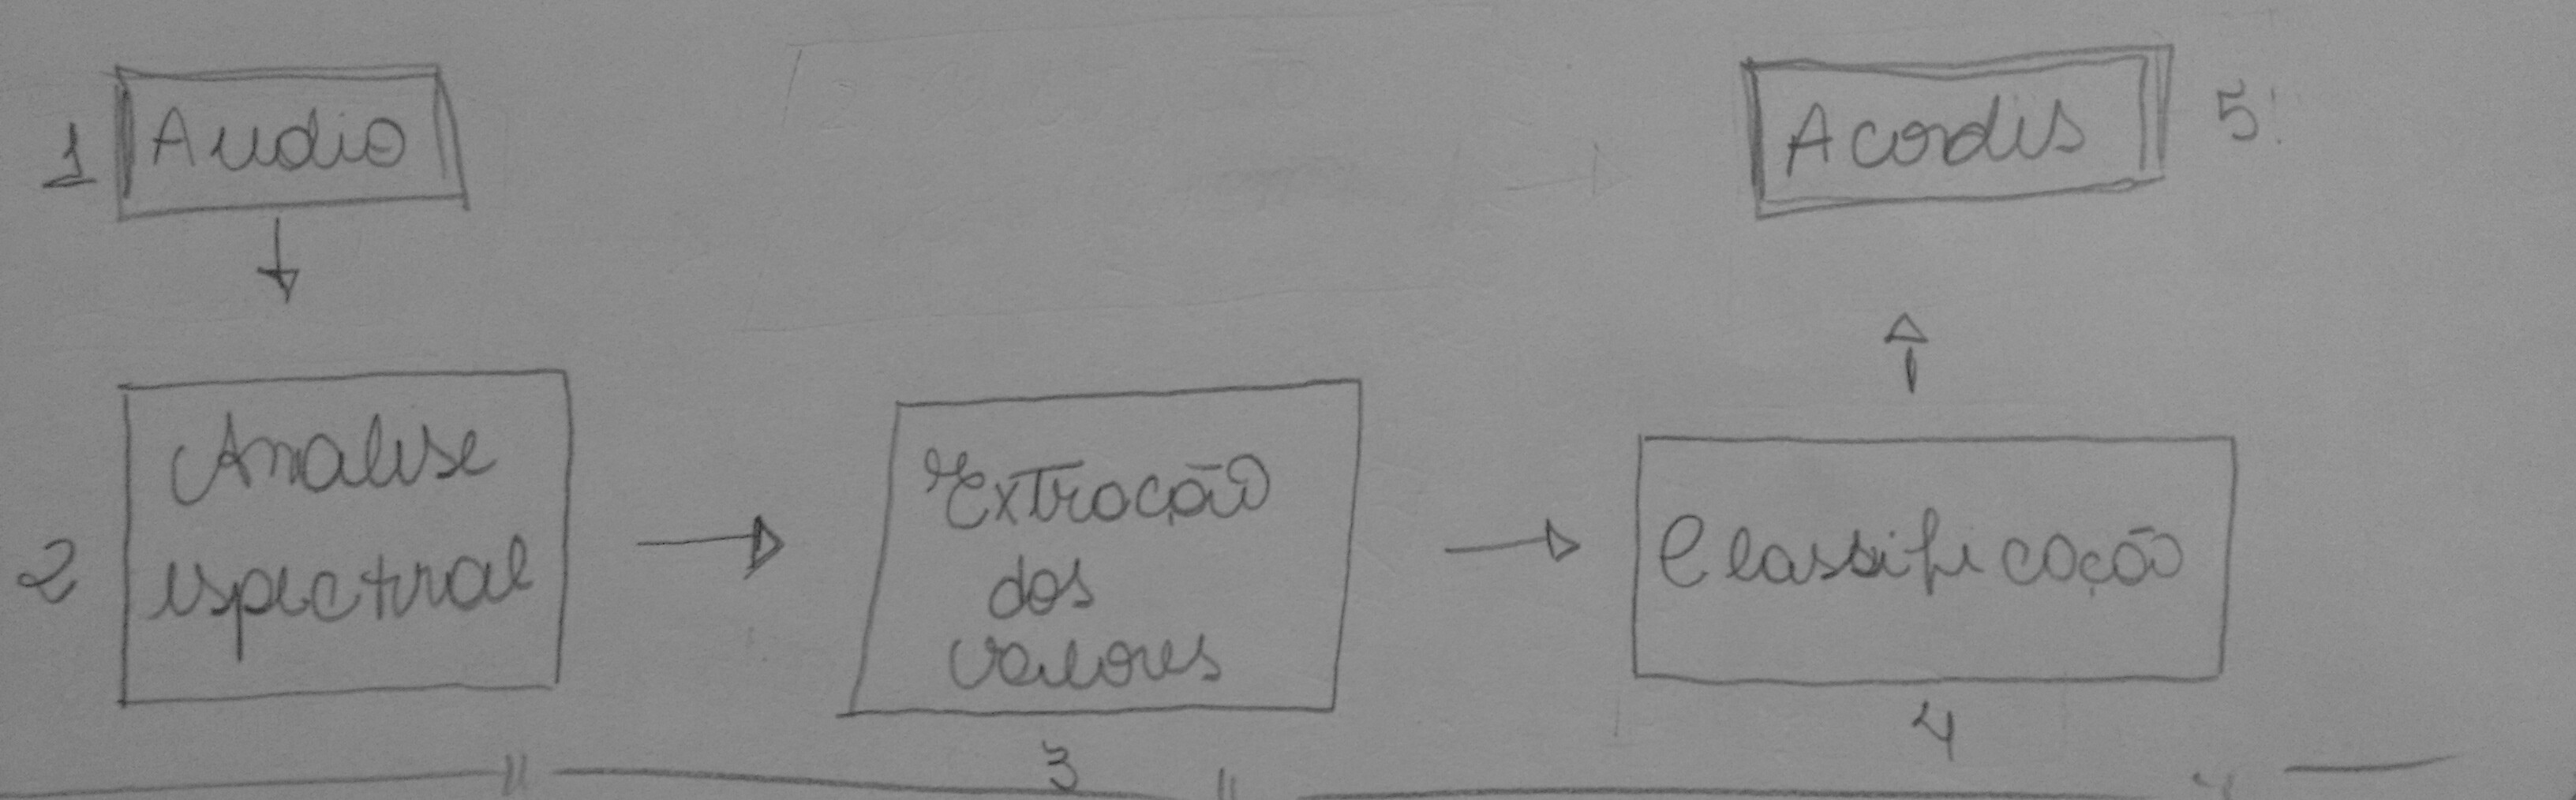
\includegraphics[scale=0.15]{figuras/IMG_20171110_144014.jpg}
     \caption{Diagrama da Metodologia}
     \label{metodologia}
\end{figure} 

% OBS: vou criar essa figura ainda

\section{Áudio}
\label{cap:audio}
Para que uma frenquência seja compreendida pelo ouvido humano, ela precisa ser repetida periodica. Por isso a entrada de áudio no formato WAVE, precisa ser fracionada e repetida perioticamente, essa quebra no audio é necessário para que se possa realizar uma analise espectral dessa frequência usando transformada rapida de Fourier.


\section{Analise Espectral}
\label{cap:analise:espectral}
Aplicamos transformada rapida de Fourier ao sinal de entrada pois precisamos trazer o audio de dominio do tempo, para o domínio da frequência, a saida dessa aplicação é o espctro de Fourier, onde conseguimos observar as notas separadamente e assim podemos armazenar esses dados nos vetores croma.


\section{Extração de Valores}
\label{cap:extraçaõ:valores}
Para construção dos vetores croma é necessário uma nota inicial F0.
Sendo F0 uma das notas temperadas da tabela de acordes. Podemos obter essa nota atraves de uma equação pré definida.
Que no caso não definimos ainda, pois não foram realizados testes nessa etapa do trabalho.

Com base no espectro de Fourier obtido através da Transformada rapida de Fourier separamos as faixas de frequência em torno da F0. 
O tamanho das faixas é um ponto importante, elas não podem ser grandes demais,pois corremos o risco de englobarem frequências intermediárias, que não nos interessam e também não podem ser muito pequenas, pois não incluiriam pequenas desafinações. Somos assim obrigados a encontrar uma solução de compromisso entre robustez e seletividade.
Para introduzirmos essa robutez desejada podemos manipular um pouco a largura dessa faixa, deixando ela um pouco mais larga que a faixa de frequencia sugerida pela F0, pois assim podemos eliminar ruidos. Sendo eles, vozes no fundo, mudanças de corda de nilon e corda de aço ou desafinação do instrumento.

Após a detecção das faixas de frequência utilizaremos da técnica de extração de picos do espectro de Fourier para construção do vetor croma, como mostra o exemplo da  \cref{extracaoPicos}.

\begin{figure}[!htb]
     \centering
     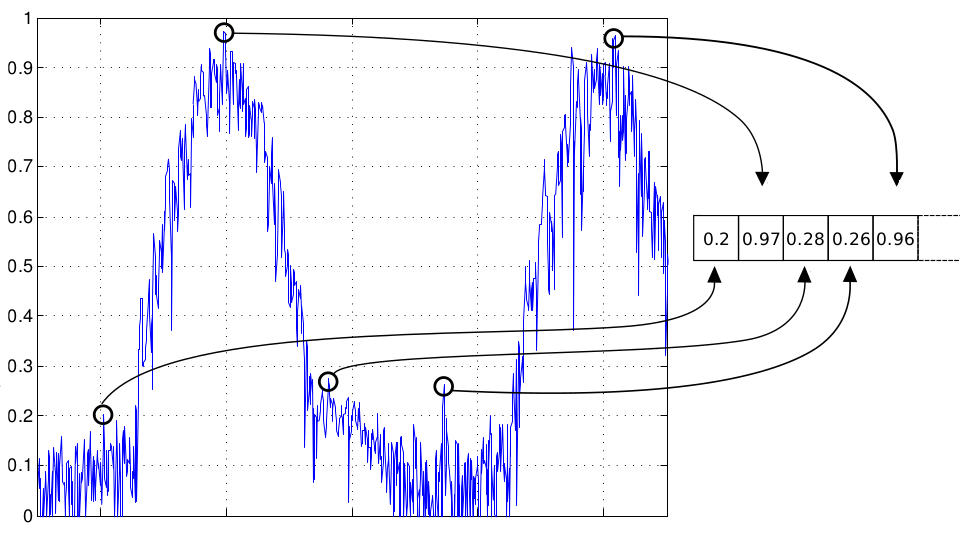
\includegraphics[scale=0.5]{figuras/picos2.png}
     \caption{Extração de picos do espectro de Fourier}
     \label{extracaoPicos}
\end{figure} 


\section{Classificador}
\label{cap:classificador}

A proposta de classificação de acordes poderá ser feita através de redes neurais artificial.
Onde usaremos uma base de dados utilizando musicas de dominio publico, com essa base de dados faremos o teste, o treinamento e a validação da rede neural artificial.

As amostras de teste e treinamento, seriam baseadas na tabela de 12 acordes e suas variações (formas diferentes de se tocar uma mesma nota) para cada acorde. 
Repetindo esses acordes para um violao com corda de aço e um violao com corda de nilon.
Podemos assim ter uma probabilidade de acerto maior para os acordes referentes ao audio de entrada.

Apos o uso dessa base de dados, podemos então aplicar essa rede neural, treinada, testada e validada nos vetores croma, para assim definirmos quais são os acordes presentes nesses vetores de croma.

Qual rede neural artificial será usado nesse trabalho ainda não foi definido, pois precisamos realizar testes para identificarmos qual rede neural teria uma porcentagem de acerto melhor para essa proposta.

\section{Acordes}
\label{cap:acrodes}
Apos aplicação das redes neurais artificias como metodo de classificação, esperamos que a saída desse sistema contenha o acorde referente ao sinal de frequência de entrada;


%---------------------------------------------------%
% \section{Considerações Finais}
% \label{cap:metodologia:sec:consideracoes:finais}

% Esta é uma sugestão de seção para dar um fechamento em cada uma dos capítulos.

% (ATENÇÃO - veja com o seu orientador se é uma seção necessária (pois trate-se de estilo de escrita))